\section{Introduction}
The challenges at hadron collider experiments are many, one of the
most well known is the fact the the energy and momentum of the parton-parton
(hard) interaction is not know. This limitation, in addition with the
fact that a large number of the proposed extensions of the SM (e.g. SUSY) predict
new particles that are weakly interacting and therefore escape the
detector systems without a trace, have made events with large momentum
imbalance in the plane transverse to the beam a key signature to
search for BSM physics. The momentum imbalance is the transverse plane
(missing energy)
is quantified by $\ptvecmiss$  which is defined as 
\begin{equation}
\label{eq:ptmiss}
\ptvecmiss = -\sum\limits_{i=0}^{n_{pf}} \vec{p}_{T}^{\hspace{0.06cm}i},
\end{equation}
where $\vec{p}_{T}^{\hspace{0.06cm}i}$ is the measured transverse
momentum of a PF candidate, and $n_{pf}$ is the total number of PF
candidates reconstructed.

Additionally, in SUSY models with R-parity conservation the originally
pair produced super-partners undergo a cascade decay and at least two
particles (the LSPs) will escape detection and therefore further reduce the
ability to fully reconstruct the event kinematics due to the lost
information. Subsequently, all these effects result in lost of
sensitivity as the discrimination power between a possible
signal and the SM background processes is reduced. In order to recover
sensitivity, different kinematic variables are employed which are
functions of the visible objects momenta and the $\ptvecmiss$. These
kinematic variables have been shown to improve signal to background
discrimination but are often model dependent. One example of such
variables are the razor variables~\cite{rogan,razor2010}, which have been widely used by the
CMS collaboration to search for
SUSY~\cite{Chatrchyan:2014goa,Razor8TeV} and recently shown to have
good sensitivity for DM direct production at hadron
colliders~\cite{Fox:2012ee}. The razor variables: $\MR$ and $\RR^2$  provide an estimate of the
underlying mass scale of the event and a handle to significantly
suppress SM backgrounds -- particularly QCD multijet --,
respectively. 

Since the two searches for BSM physics presented in this thesis are
based on the razor variables, this Chapter describes its derivation
(see Section~\ref{razorVariables})
and their main features when searching for new physics (see Section~\ref{razorApp}).

\section{The Razor Variables}\label{razorVariables}
The razor variables were originally derived~\cite{rogan,razor2010} for
squark pair-production in the context of SUSY; this topology is
represented by the Feynman diagram shown in Figure~\ref{fig:squarkpair}, where
the proton-proton collision pair produces two squarks ($\tilde{q}_{1}\tilde{q}_{2}$) which
subsequently decay into a SM quark and the LSP ($\tilde{q}_{i}\rightarrow q_{i}\tilde{\chi}_{1}^{0}$).

\begin{figure}
 \centering
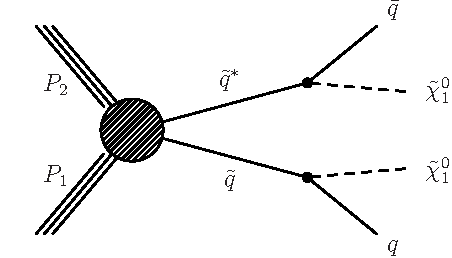
\includegraphics[width=0.4\textwidth]{RazorVariables/T2qq.pdf}
 \caption{Feynman diagram for squark pair-production.\label{fig:squarkpair}}
\end{figure}
One interesting quantity that provides access to the mass scale of the
SUSY particles is the magnitude of the 3-momentum of the quark in the
rest frame of the squark, it is actually more convenient to write down
twice this quantity:
\begin{equation}
\label{eq:pq}
2|\vec{p}^{\hspace{0.06cm}q_{i}}| =
2|\vec{p}^{\hspace{0.06cm}\tilde{\chi}_{1}^{0}}| =
\frac{\sqrt{m^{4}_{\tilde{q}} -
2m^{2}_{\tilde{q}}m^{2}_{\tilde{\chi}_{1}^{0}} +
m^{4}_{\tilde{\chi}_{1}^{0}} - 2m^{2}_{q}m^{2}_{\tilde{\chi}_{1}^{0}}
- 2m^{2}_{q}m^{2}_{\tilde{q}} + m_{q}^{4}}}{m_{\tilde{q}}},
\end{equation}
 where $m_{\tilde{q}}$ is the squark mass, $m_{\tilde{\chi}_{1}^{0}}$
 is the LSP mass, and $m_{q}$ is the SM quark mass. Eq.~\ref{eq:pq}
 can be simplified if the SM quarks are assumed massless -- which is
 mostly accurate with the exception of the top-quark. This
 simplification is also useful to define:
\begin{equation}
\label{eq:Mdelta}
M_{\Delta} = 2|\vec{p}^{\hspace{0.06cm}q_{i}}| =
\frac{m^{2}_{\tilde{q}} -
m^{2}_{\tilde{\chi}_{1}^{0}}}{m_{\tilde{q}}}.
\end{equation}

$M_{\Delta}$ is sensitive to the mass-splitting between the squark and
the LSP  and therefore is usually refer to as the characteristic mass
scale of the event. For example, in the case of the $W\rightarrow
\ell\nu$ decay, $M_{\Delta}$ is simply the mass of the W boson.

The razor variable \MR provides an estimate of $M_{\Delta}$ by
approximating the boosts needed -- since the actual boosts are
impossible to reconstruct due to the missing particles, which can be
viewed as an undetermined system of equations with not enough
constraints -- to go from the laboratory frame (lab frame) to the
squark rest frame. This approximation is done in two steps, first
, there is a common boost to go from the lab frame to the
center-of-momentum (CM) frame, and then, an equal and opposite boost
applied to each squark to go from the CM frame to their respective
rest frame. Figure~\ref{fig:restFrames} depicts the three frames and
the boosts needed to move from the lab frame to the squark rest frames.
\begin{figure}
 \centering
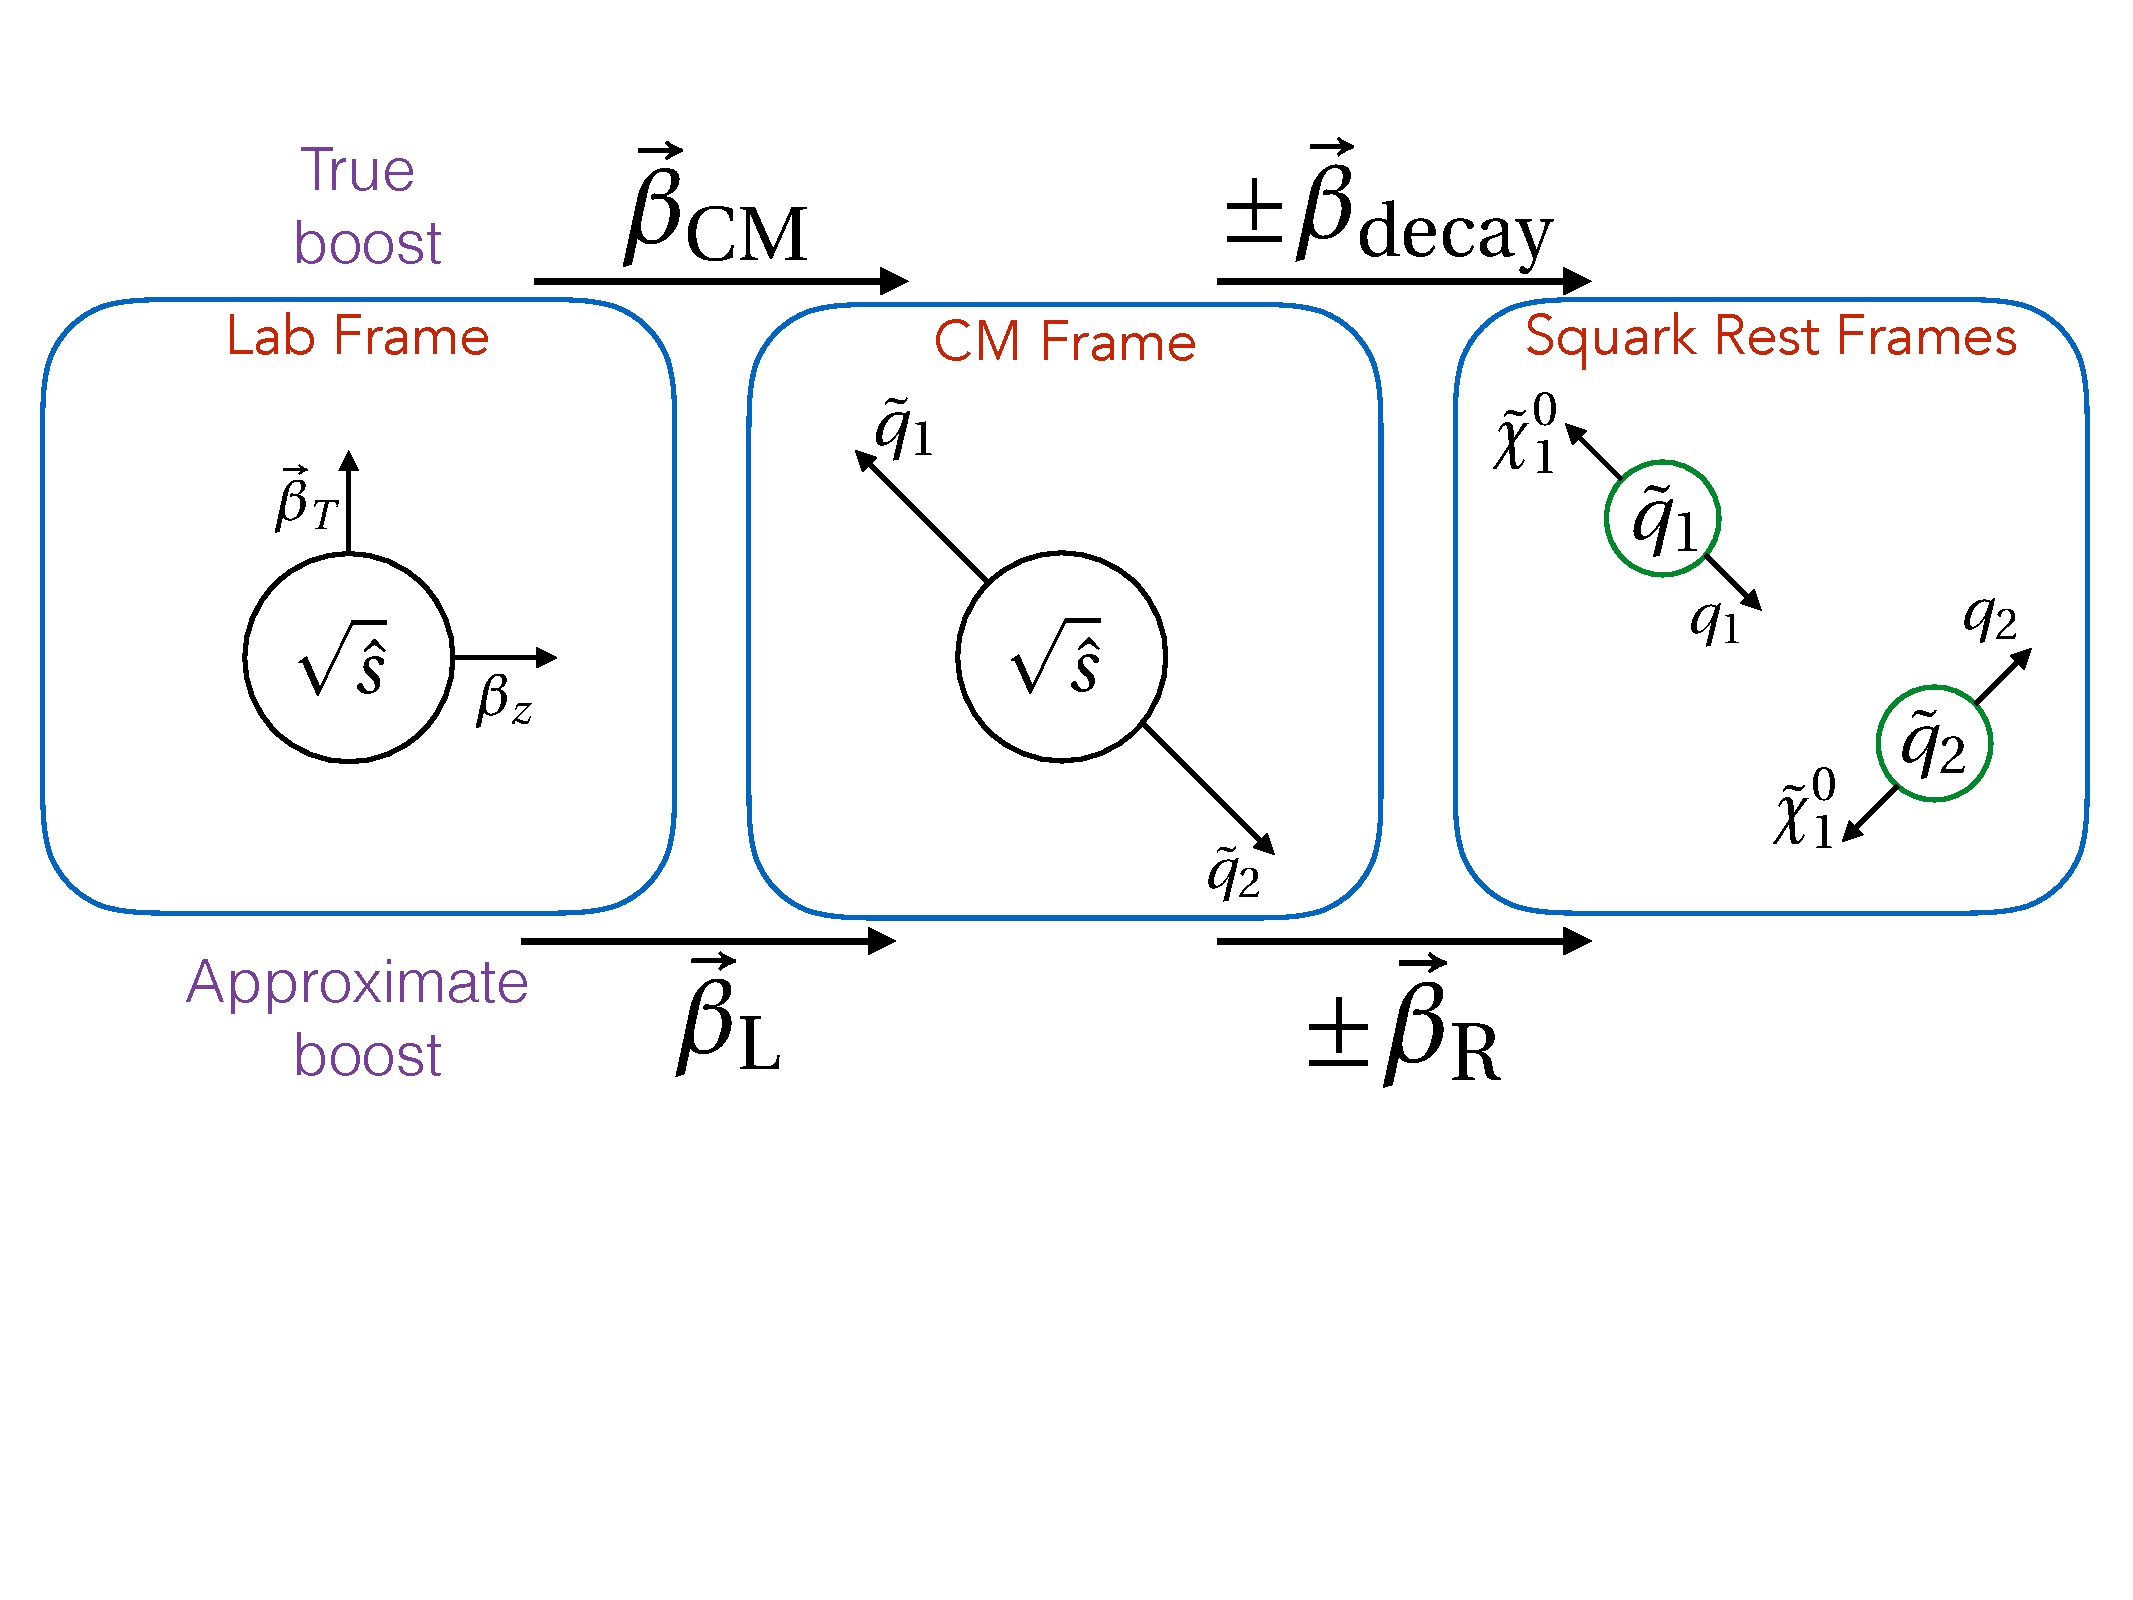
\includegraphics[width=1.0\textwidth]{RazorVariables/RazorFrameDiagram.pdf}
 \caption{An schematic of the  different rest frames involved in
   deriving the razor variables. The lab frame is in the left panel,
   the CM frame is in the middle panel, and the  squark rest frames
   are in the right panel.\label{fig:restFrames}}
\end{figure}  

The approximate boost relating the CM frame and the rest frames of each of the
squarks ($\vec{\beta}_{R}$) is asymmetric since the two squarks are recoiling against each
other in the CM frame. $\vec{\beta}_{R}$ is obtained by adding the condition
that in their respective squark rest frame the magnitude of each quark
momentum is the same, this is to say that the two decays are identical
up to the decay angle. Since the quarks are assumed to be massless
the condition is:

\begin{equation}
\label{eq:razorCond1}
E^{q_{1}}_{s} = E^{q_{2}}_{s}
\end{equation}
\begin{equation}
\label{eq:razorCond11}
\Rightarrow\gamma_{R}(E^{q_{1}}_{CM} -\vec{\beta}_{R} \cdot \vec{p}_{CM}^{\hspace{0.06cm}q_{1}})= \gamma_{R}(E^{q_{2}}_{CM} +\vec{\beta}_{R} \cdot \vec{p}_{CM}^{\hspace{0.06cm}q_{2}})
\end{equation}
\begin{equation}
\label{eq:razorCond12}
\Rightarrow\vec{\beta}_{R} \cdot (\vec{p}_{CM}^{\hspace{0.06cm}q_{1}}+\vec{p}_{CM}^{\hspace{0.06cm}q_{2}})= E^{q_{1}}_{CM} -E^{q_{2}}_{CM},
\end{equation}

where $E^{q_{i}}_{s}$ is the energy of the $i$-th quark on its
respective squark rest frame, $E^{q_{i}}_{CM}$ is the energy of the
$i$-th quark in the CM frame, $\vec{p}_{CM}^{\hspace{0.06cm}q_{i}}$ is the momentum of the
$i$-th quark in the CM frame, and $\gamma_{R}$ is the gamma factor
corresponding to $\vec{\beta}_{R}$. This symmetry constraint is not
enough to uniquely determine $\vec{\beta}_{R}$ and therefore an
external condition is required; this external condition is such that
the boost minimizes the sum of the quarks energies, i.e.

\begin{equation}
\label{razonMinCondition}
\frac{\partial (E^{q_{1}}_{s} + E^{q_{2}}_{s})}{\partial
  \vec{\beta}_{R}} = 0.
\end{equation}

With the addition of this extremal condition, the boost is now
found to be
\begin{equation}
\label{razonRboost}
  \vec{\beta}_{R}  = \frac{\vec{p}_{CM}^{\hspace{0.06cm}q_{1}}-\vec{p}_{CM}^{\hspace{0.06cm}q_{2}}}{E^{q_{1}}_{CM} + E^{q_{2}}_{CM}}.
\end{equation}


Now, let's turn to the boost that relates the CM and the lab
frames. The later is approximated by a
purely longitudinal boost ($\vec{\beta}_{L} = \beta_{L} \cdot \hat{z}$). Again, the assumption that the boost is in the longitudinal
direction only is not enough to uniquely determine $\beta_{L}$ and
therefore an additional constraint is needed. We require that the
longitudinal momentum of the visible system in the CM frame ought to
be zero -- only resembling the true constraint: that the sum of the visible
and invisible systems is indeed zero. This additional constraint, 
\begin{equation}
\label{eq:razorCond2}
p^{1z}_{CM} + p^{2z}_{CM} = 0,
\end{equation}
is sufficient to find the magnitude of the boost :
\begin{equation}
\label{razonLboost}
  \vec{\beta}_{L}  = \frac{p^{1z}_{\ell} + p^{2z}_{\ell}}{E^{q_{1}}_{\ell} + E^{q_{2}}_{\ell}}.
\end{equation}

With both boost now found, the only remaining task is to transform the
quantities in the squark rest frame to the lab frame to be able to use
them in a realistic environment. We define the characteristic mass
estimator ($\mathrm{M_{R}}$), which is
related to $M_{\Delta}$, in the following fashion: 
\begin{equation}
\label{eq:MRdef}
\mathrm{M_{R}} \equiv \gamma_{R}(E^{q_{1}}_{s} + E^{q_{2}}_{s}) =
  \gamma_{R} M_{\Delta}.
\end{equation} 

When expressed in the corresponding lab frame quantities by applying
the boosts just found above, $\mathrm{M_{R}}$ takes the form:

 \begin{equation}
\label{eq:MRlabF}
\mathrm{M_{R}} = \sqrt{(E^{q_{1}}_{\ell} + E^{q_{2}}_{\ell})^{2} - (p^{1z}_{\ell} + p^{2z}_{\ell})^{2}}.
\end{equation} 


We now proceed to construct another variable purely from the
transverse information in the detector. Inspired by the ideal
back-to-back topology of QCD dijet events we define the razor
transverse mass variable:

\begin{equation}
\label{eq:MRTdef}
\mathrm{M^{R}_{T}} =
\sqrt{\frac{E^{\mathrm{miss}}_{\mathrm{T}}(p^{q_{1}}_{\mathrm{T}}+p^{q_{2}}_{\mathrm{T}})
    - \ptvecmiss \cdot (\vec{p}^{q_{1}}_{\mathrm{T}} + \vec{p}^{q_{2}}_{\mathrm{T}})}{2}}.
\end{equation} 

This variable estimates the transverse momentum imbalance in the event
and therefore is useful to discriminate between signal and
background. Additionally, $\mathrm{M^{R}_{T}}$ is strictly smaller
than $\mathrm{M_{R}}$ ( $\mathrm{M_{R}} < \mathrm{M_{R}}$), with this
in mind we define de dimensionless razor variable:

\begin{equation}
\label{eq:R2}
\mathrm{R^{2}} = \left(\frac{\mathrm{M^{R}_{T}}}{\mathrm{M_{R}} }\right)^{2}.
\end{equation}

Background events with no missing energy will tend to have values of $\mathrm{R^{2}}$ close
to zero, while signal events will have values of $\mathrm{R^{2}}$
that are on average larger than zero.


The razor variables have been also generalized to topologies which
include more than two visible objects in the detector. In order to
achieve this, a simple approach has been taken. Whenever more than two
visible objects are present, the event is forced into a dijet-like topology
by clustering all visible objects into two \textit{megajets}. All
possible permutations of these \textit{megajets} are formed
by adding the 4-momenta of the visible objects; we choose the configuration
that minimizes $M_{1}^{2} + M_{2}^{2}$, where $M_{i}$ is the mass
of the $i$-th \textit{megajet}.

\section{Application of the Razor Variables to Search for BSM Physics}\label{razorApp}

The razor variables have been employed in canonical searches for SUSY
at the LHC~\cite{razor2010,Razor8TeV,Razor13TeV} and have been shown to have good sensitivity in a variety
of final states. In this section a review of the main properties of
this variables and a summary of the main results of the searches in
references~\cite{razor2010,Razor8TeV,Razor13TeV} is given.

Let's first examine if the expected behavior of the razor variables
for the canonical squark pair production (see
Figure~\ref{fig:squarkpair}) is indeed
observed. Figure~\ref{fig:RazorVar} shows the $\mathrm{M_{R}}$ and
$\mathrm{R^{2}}$ for squark pair production in the left and right
panel, respectively. The mass of the squark was fixed to 1150\GeV and
the LSP mass was varied between 50-900\GeV. As expected,
$\mathrm{M_{R}}$ peaks a characteristic value related to
$M_{\Delta}$. For example, $M_{\Delta}$ is approximately 930\GeV when the LSP
mass is 500\GeV -- this can be calculated by just plugging in the appropriate mass values
into Equation~\ref{eq:Mdelta} -- and for this case $\mathrm{M_{R}}$ peaks at around
$\sim$1000\GeV. Additionally, $\mathrm{R^{2}}$ exhibits a falling
distribution that on average are much higher than the expected values
for the SM processes -- again, specially the daunting QCD dijet
production. Finally, Figure~\ref{fig:MRvsRsq} shows the 2-dimensional
$\mathrm{M_{R}}$-$\mathrm{R^{2}}$ distribution for the same model, but
adding contours of constant SM background. It is observed that the
signals populates very clear regions on this 2-dimensional plane and
that the SM background is reduced significantly (around 5 orders of
magnitude between the first and third contour) when more extreme
values of the razor variables are required.
\begin{figure}
 \centering
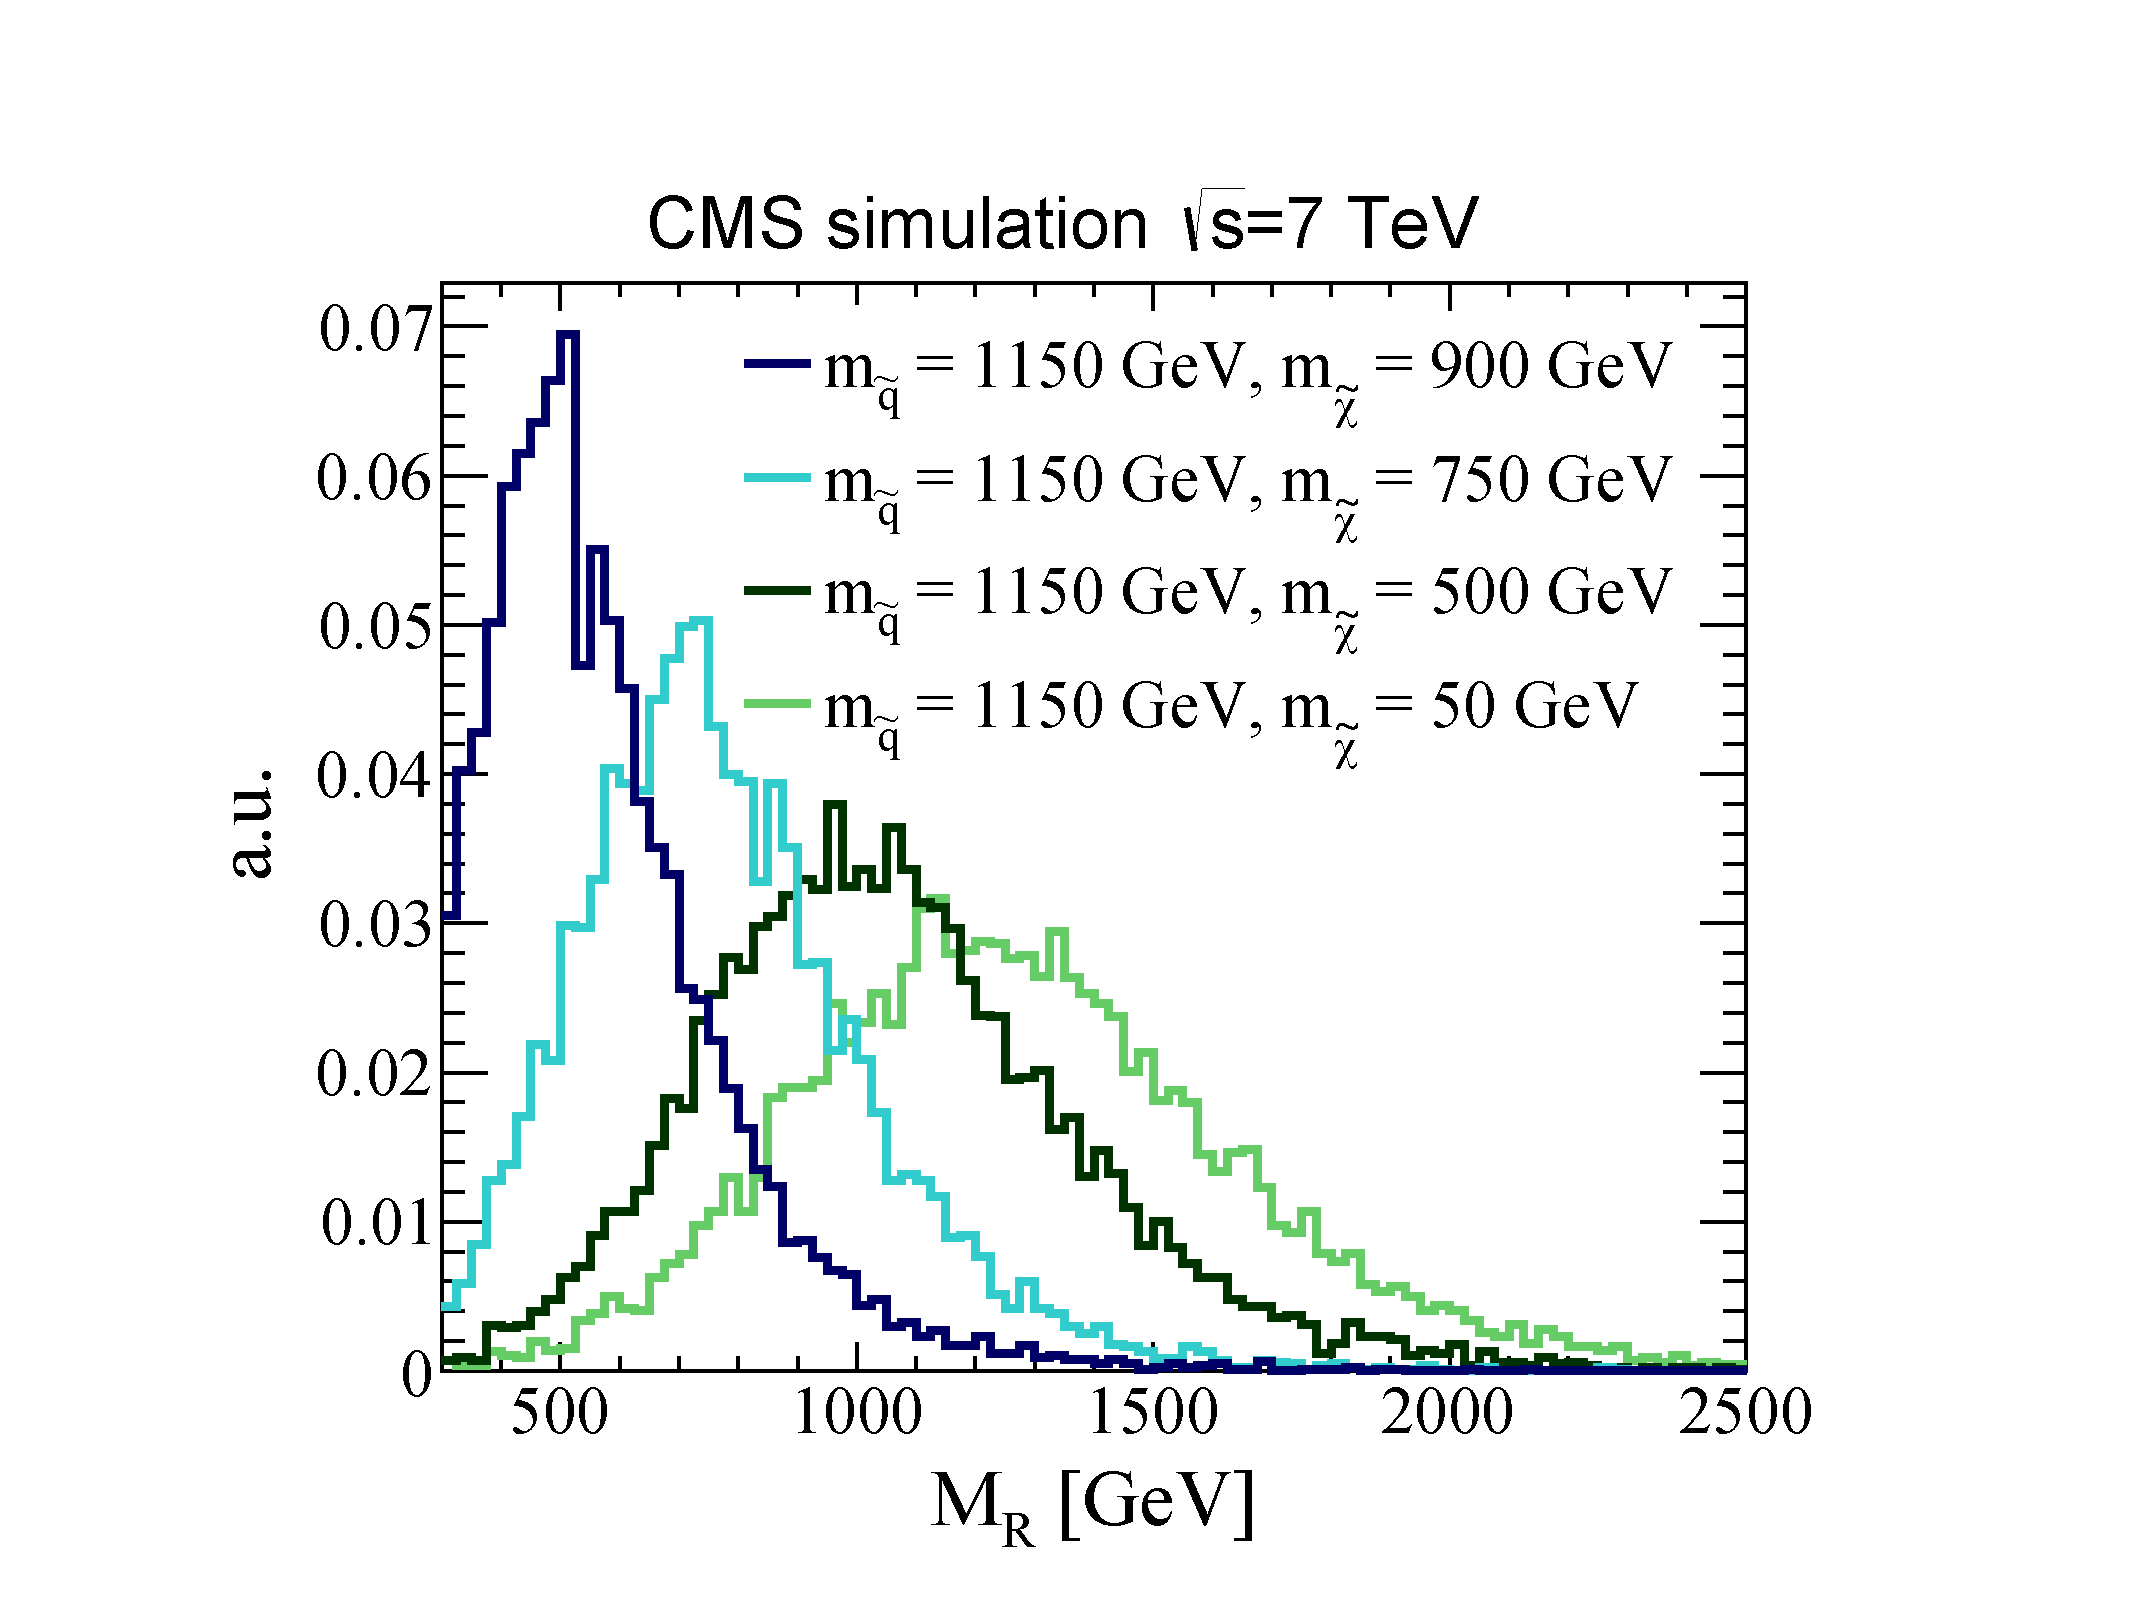
\includegraphics[width=0.49\textwidth]{RazorVariables/MR_Plot.pdf}
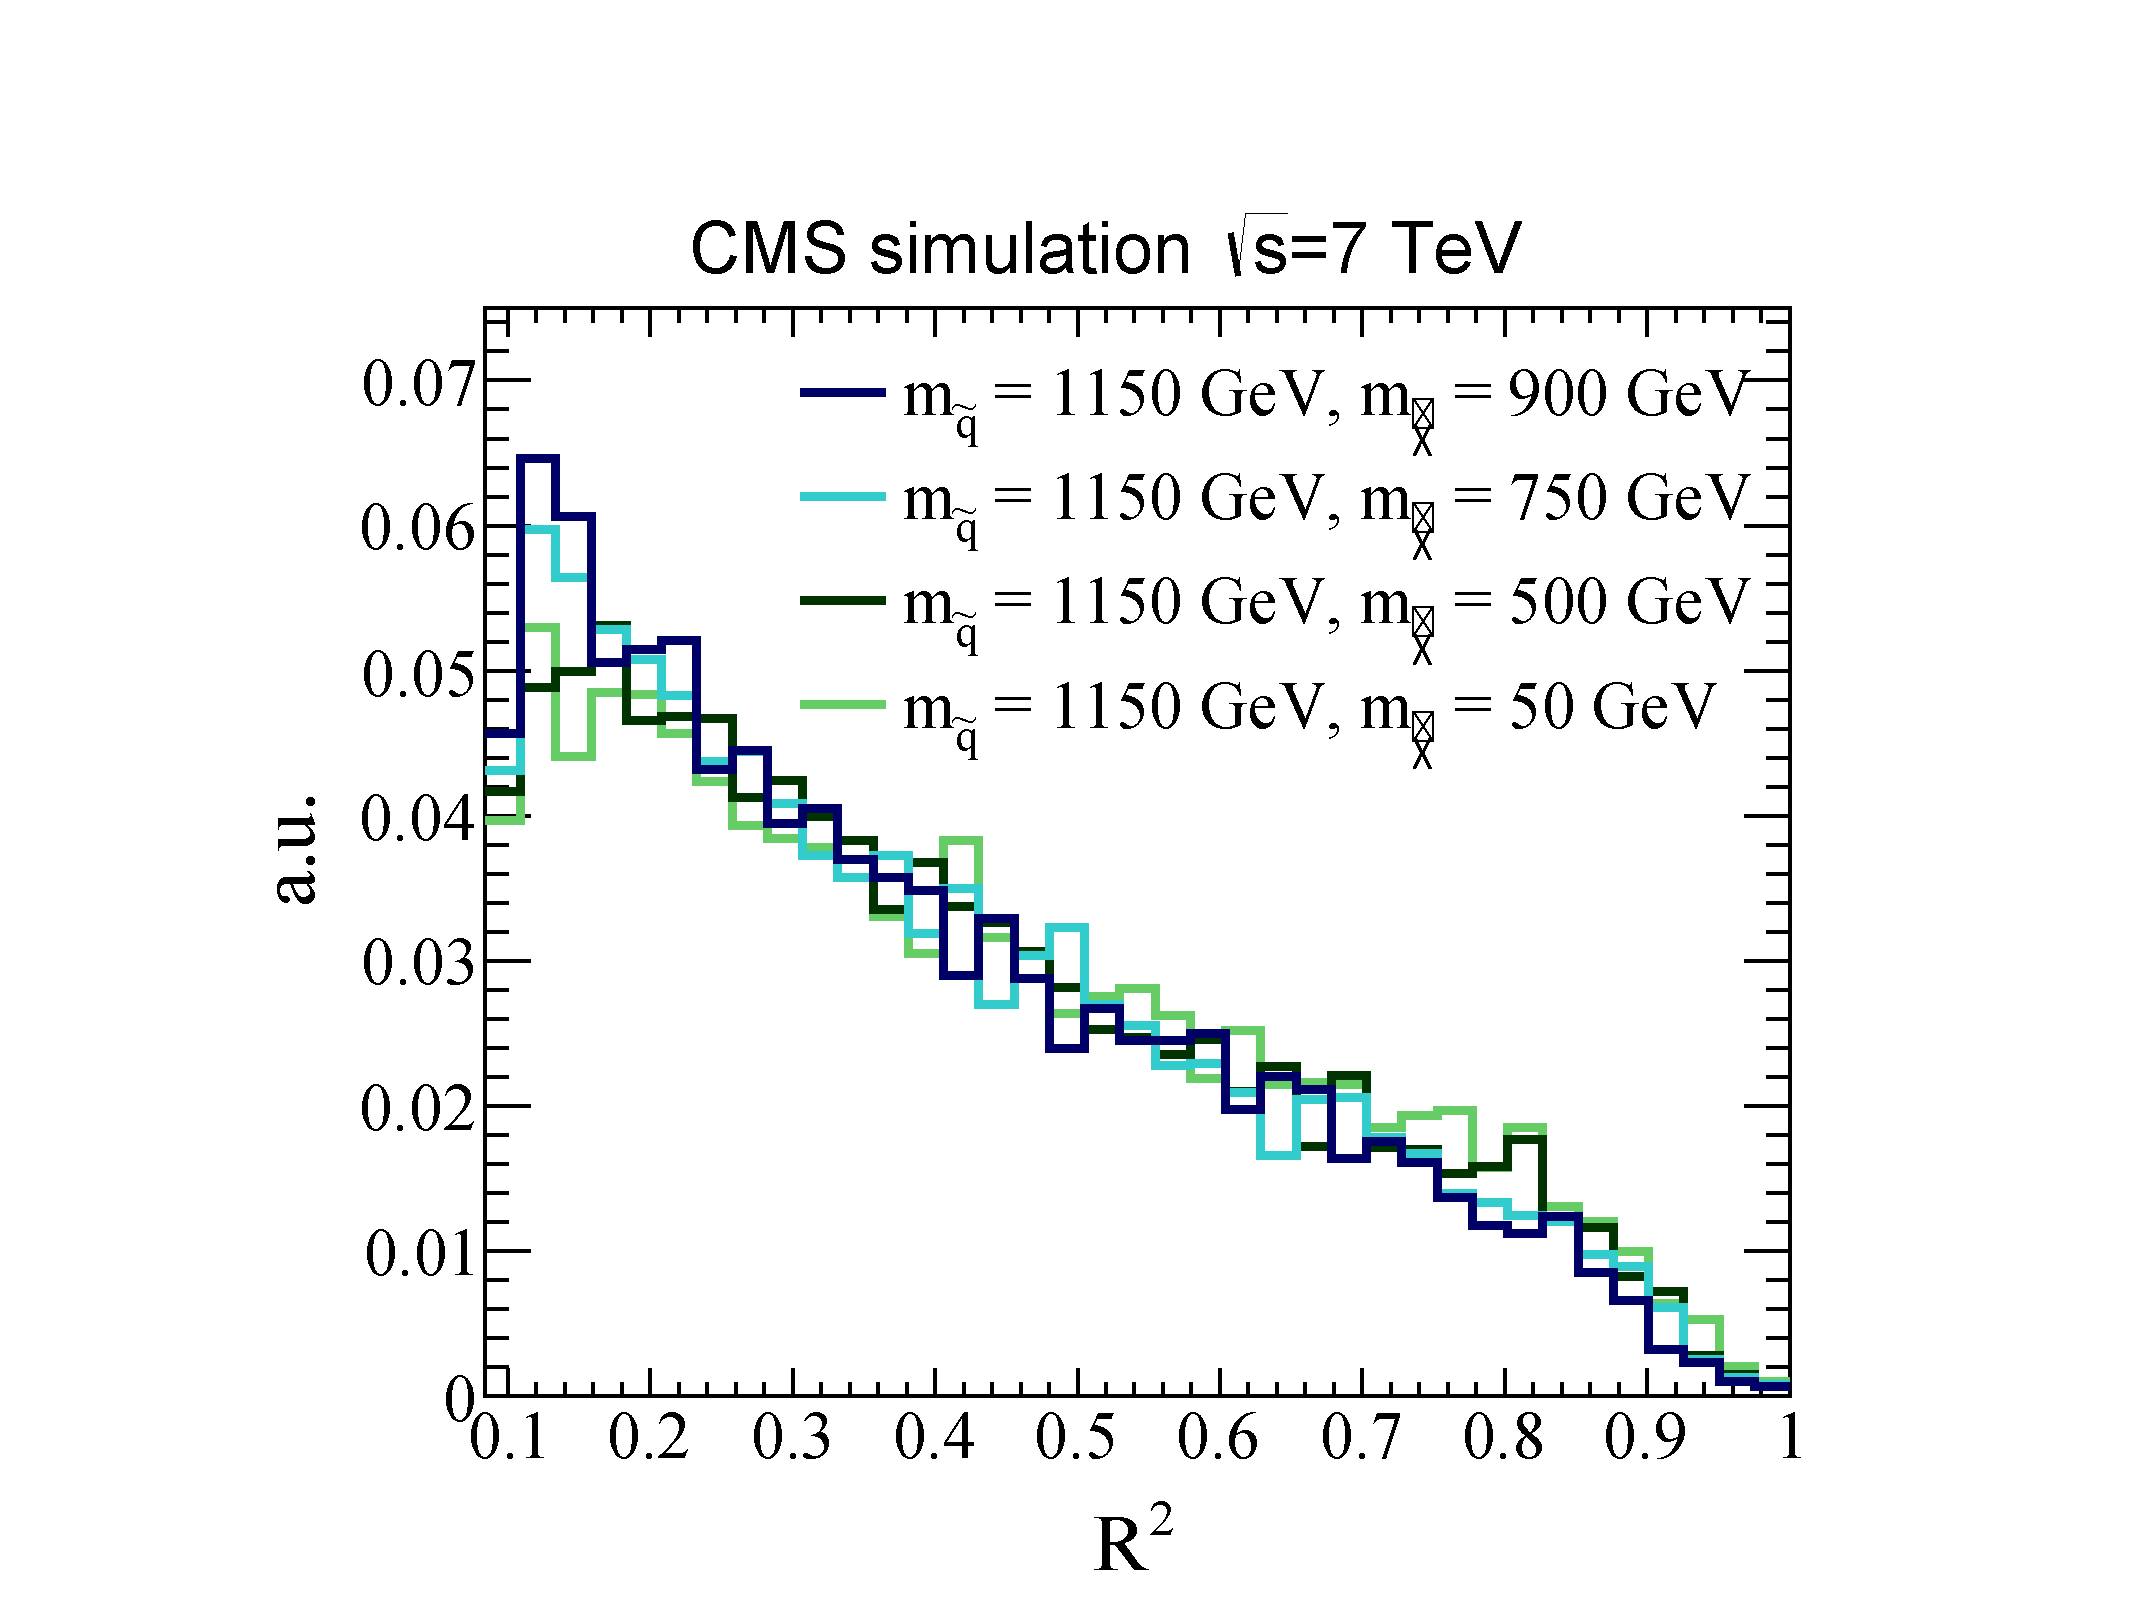
\includegraphics[width=0.49\textwidth]{RazorVariables/R2_Plot.pdf}
 \caption{Razor variables distributions for squark
   pair-production. $\mathrm{M_{R}}$ is shown in the left panel and
   $\mathrm{R^{2}}$ is shown in the right panel. The squark mass is
   set to 1150\GeV while the LSP mass is varied and shown with
   different color lines.\label{fig:RazorVar}}
\end{figure}
\begin{figure}
 \centering
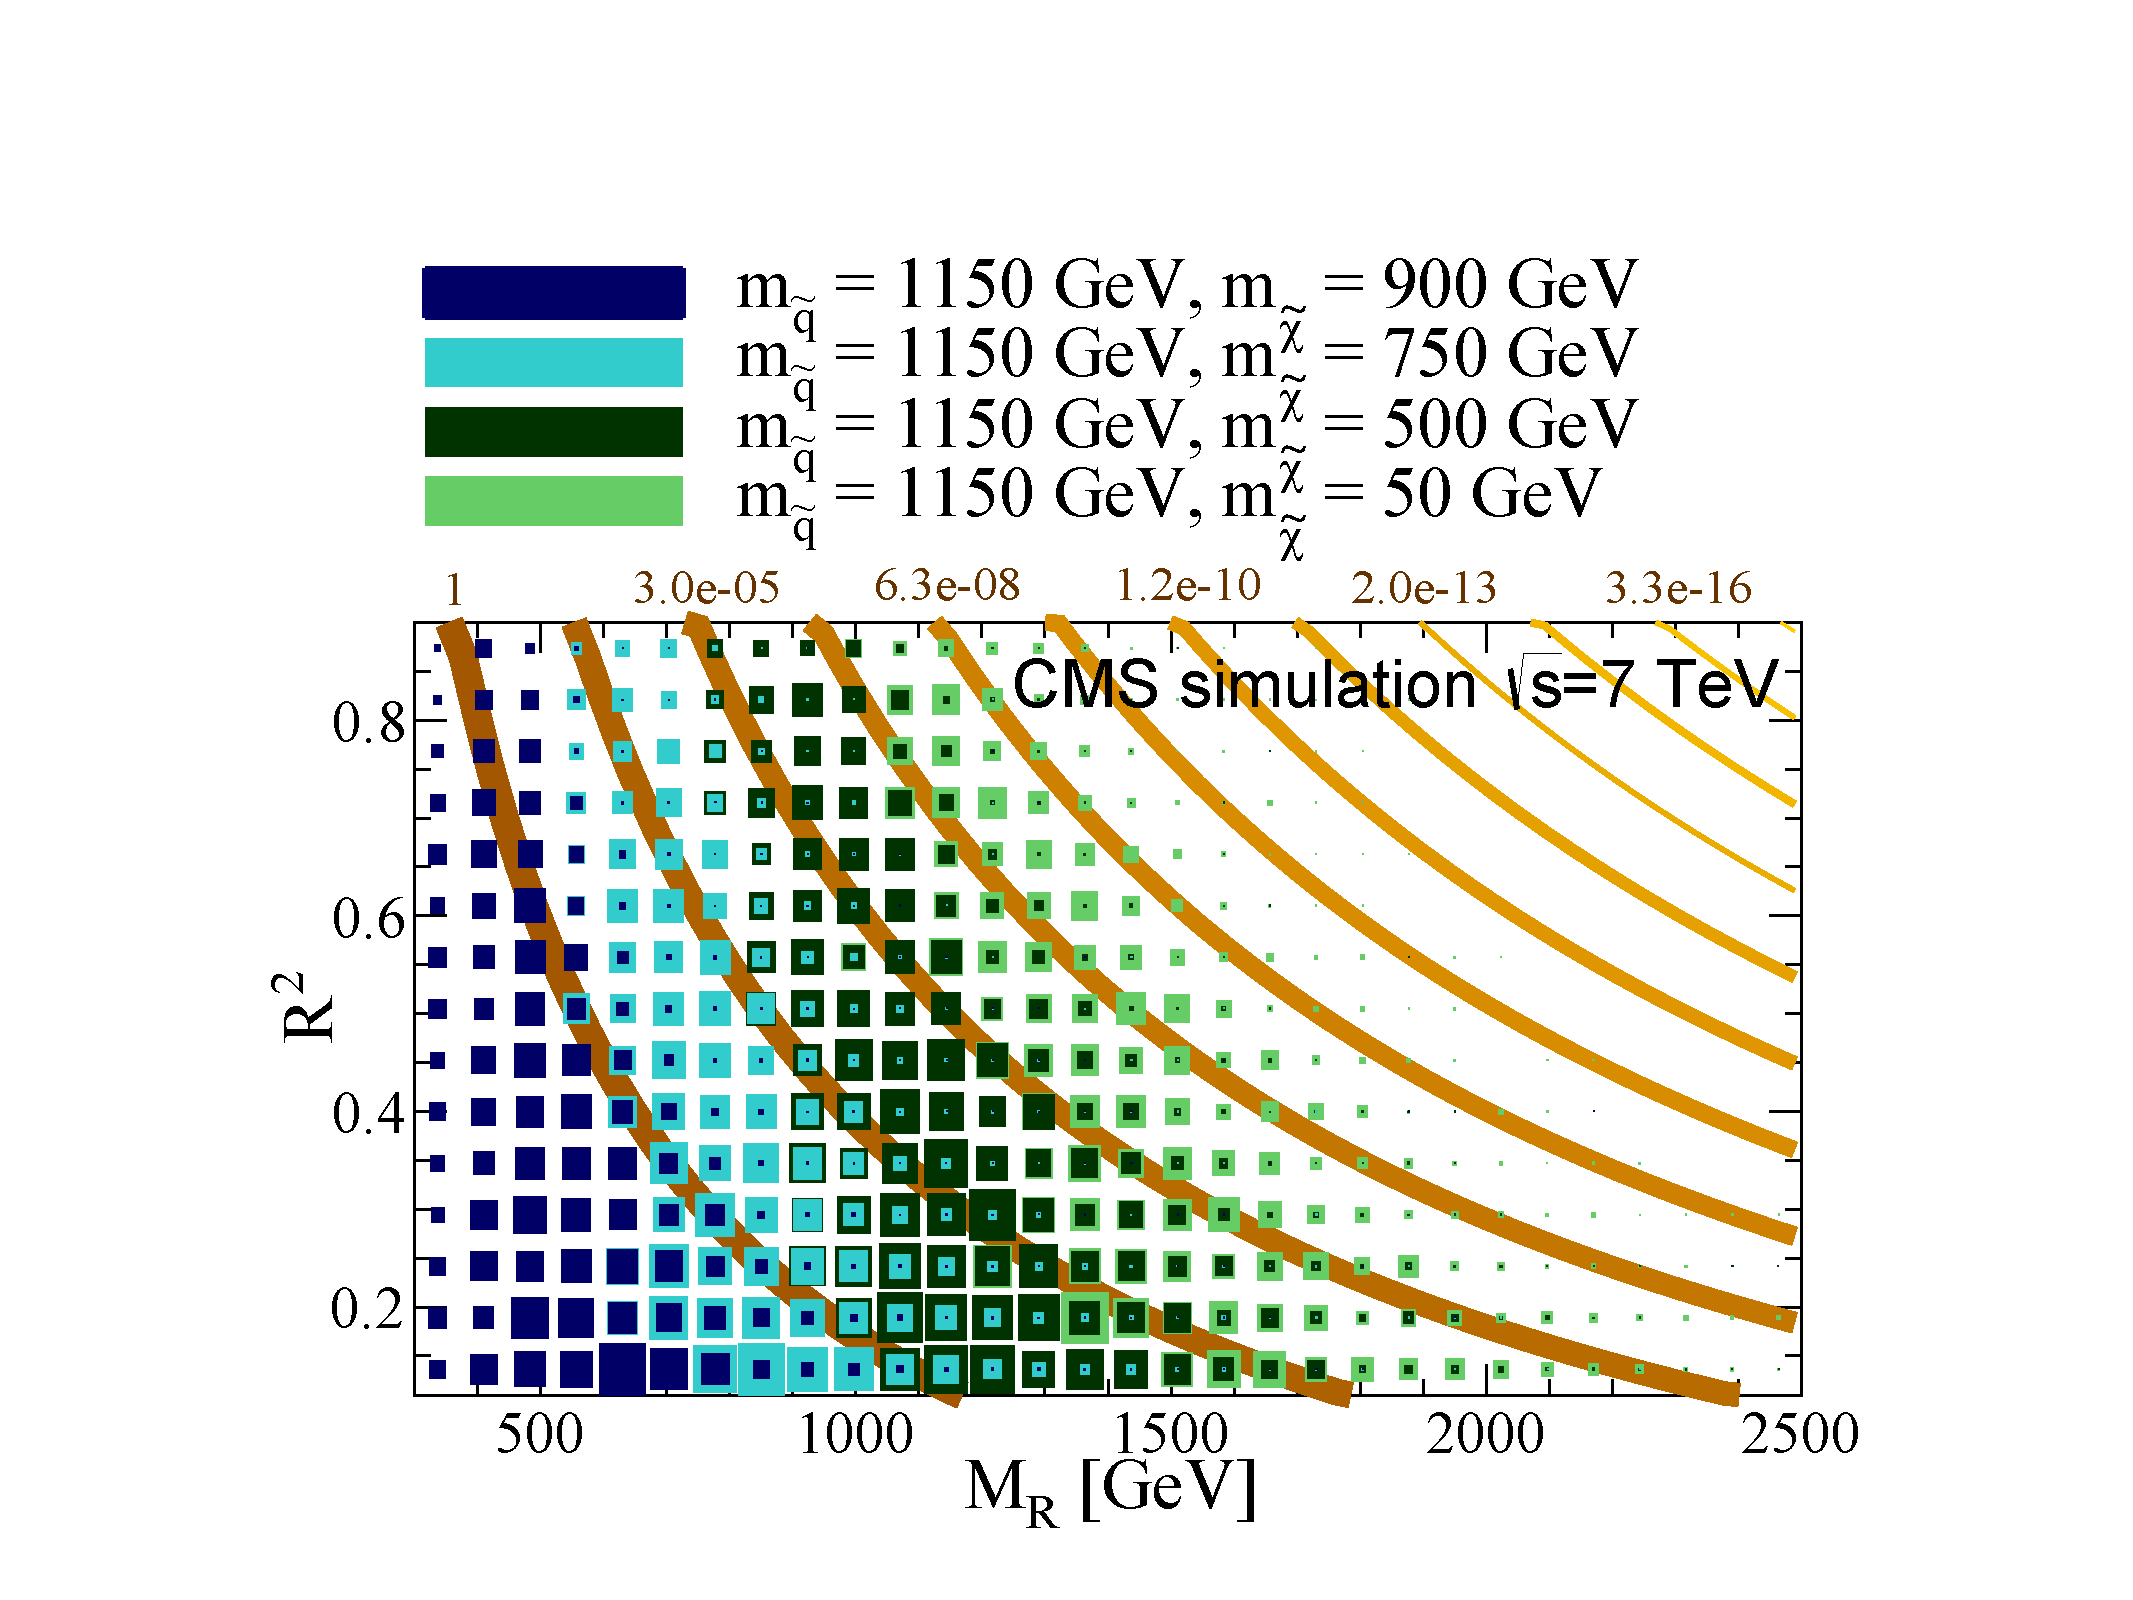
\includegraphics[width=0.7\textwidth]{RazorVariables/MR_vs_Rsq_Plot.pdf}
\caption{The 2-dimensional $\mathrm{R^{2}}$-$\mathrm{M_{R}}$
  distribution. The squark mass is
   set to 1150\GeV while the LSP mass is varied and shown with
   different color squares. The orange band represents the contour of
   constant SM background.\label{fig:MRvsRsq}}
\end{figure} 


The first result using razor variables was carried out by CMS using data
collected a center-of-mass energy of 7\TeV where an inclusive final
state approach was adopted selecting jets, b-jets, and also leptons in
the final state. There was no deviation from the SM background
estimation and 95\% confidence level (CL) limits on the CMSSM model
were placed. Figure~\ref{fig:Limit7TeV} shows the combine limit.
CMS released another search for SUSY with razor variables using the full
dataset ($\sim 20$ fb$^{-1}$) collected at 8\TeV, again, with no observed significant
deviations from the SM background estimation. It is of note that the
background estimation, which employs a fit to the sidebands of the
data using an analytical functional form, was much improved with
respect to the 7\TeV counterpart. The results were interpreted in the
context of SUSY simplified models of gluino and top-squark (stop) pair
production where the branching ratios (BRs) of the particles involved
were varied in order to produce a more general
result. Figure~\ref{fig:RazorLimit8TeV} shows the 95\% CL. limits for
gluino and stop pair-production in the left and right panels,
respectively. It is observed that the gluino is excluded around
1200-1400\GeV depending on the exact values of the BRs, and the stop is
excluded at about 700\GeV regardless of its BRs. Recently, an updated
search using the first portion of 13\TeV data ($\sim 2.1$ fb$^{-1}$) was released following
greatly the approach taken in the 8\TeV counterpart but adding an
additional and totally independent background estimation based on scale
factors derived in data control
regions. Figure~\ref{fig:RazorLimit13TeV} show the 95\% CL. limits for
gluino pair-production. It is observed that the gluino is excluded around
1400-1600\GeV depending on the exact values of the BRs. It is of note
that with only 10\% of the integrated luminosity the 13\TeV result
surpasses the corresponding 8\TeV result.
 
\begin{figure}
 \centering
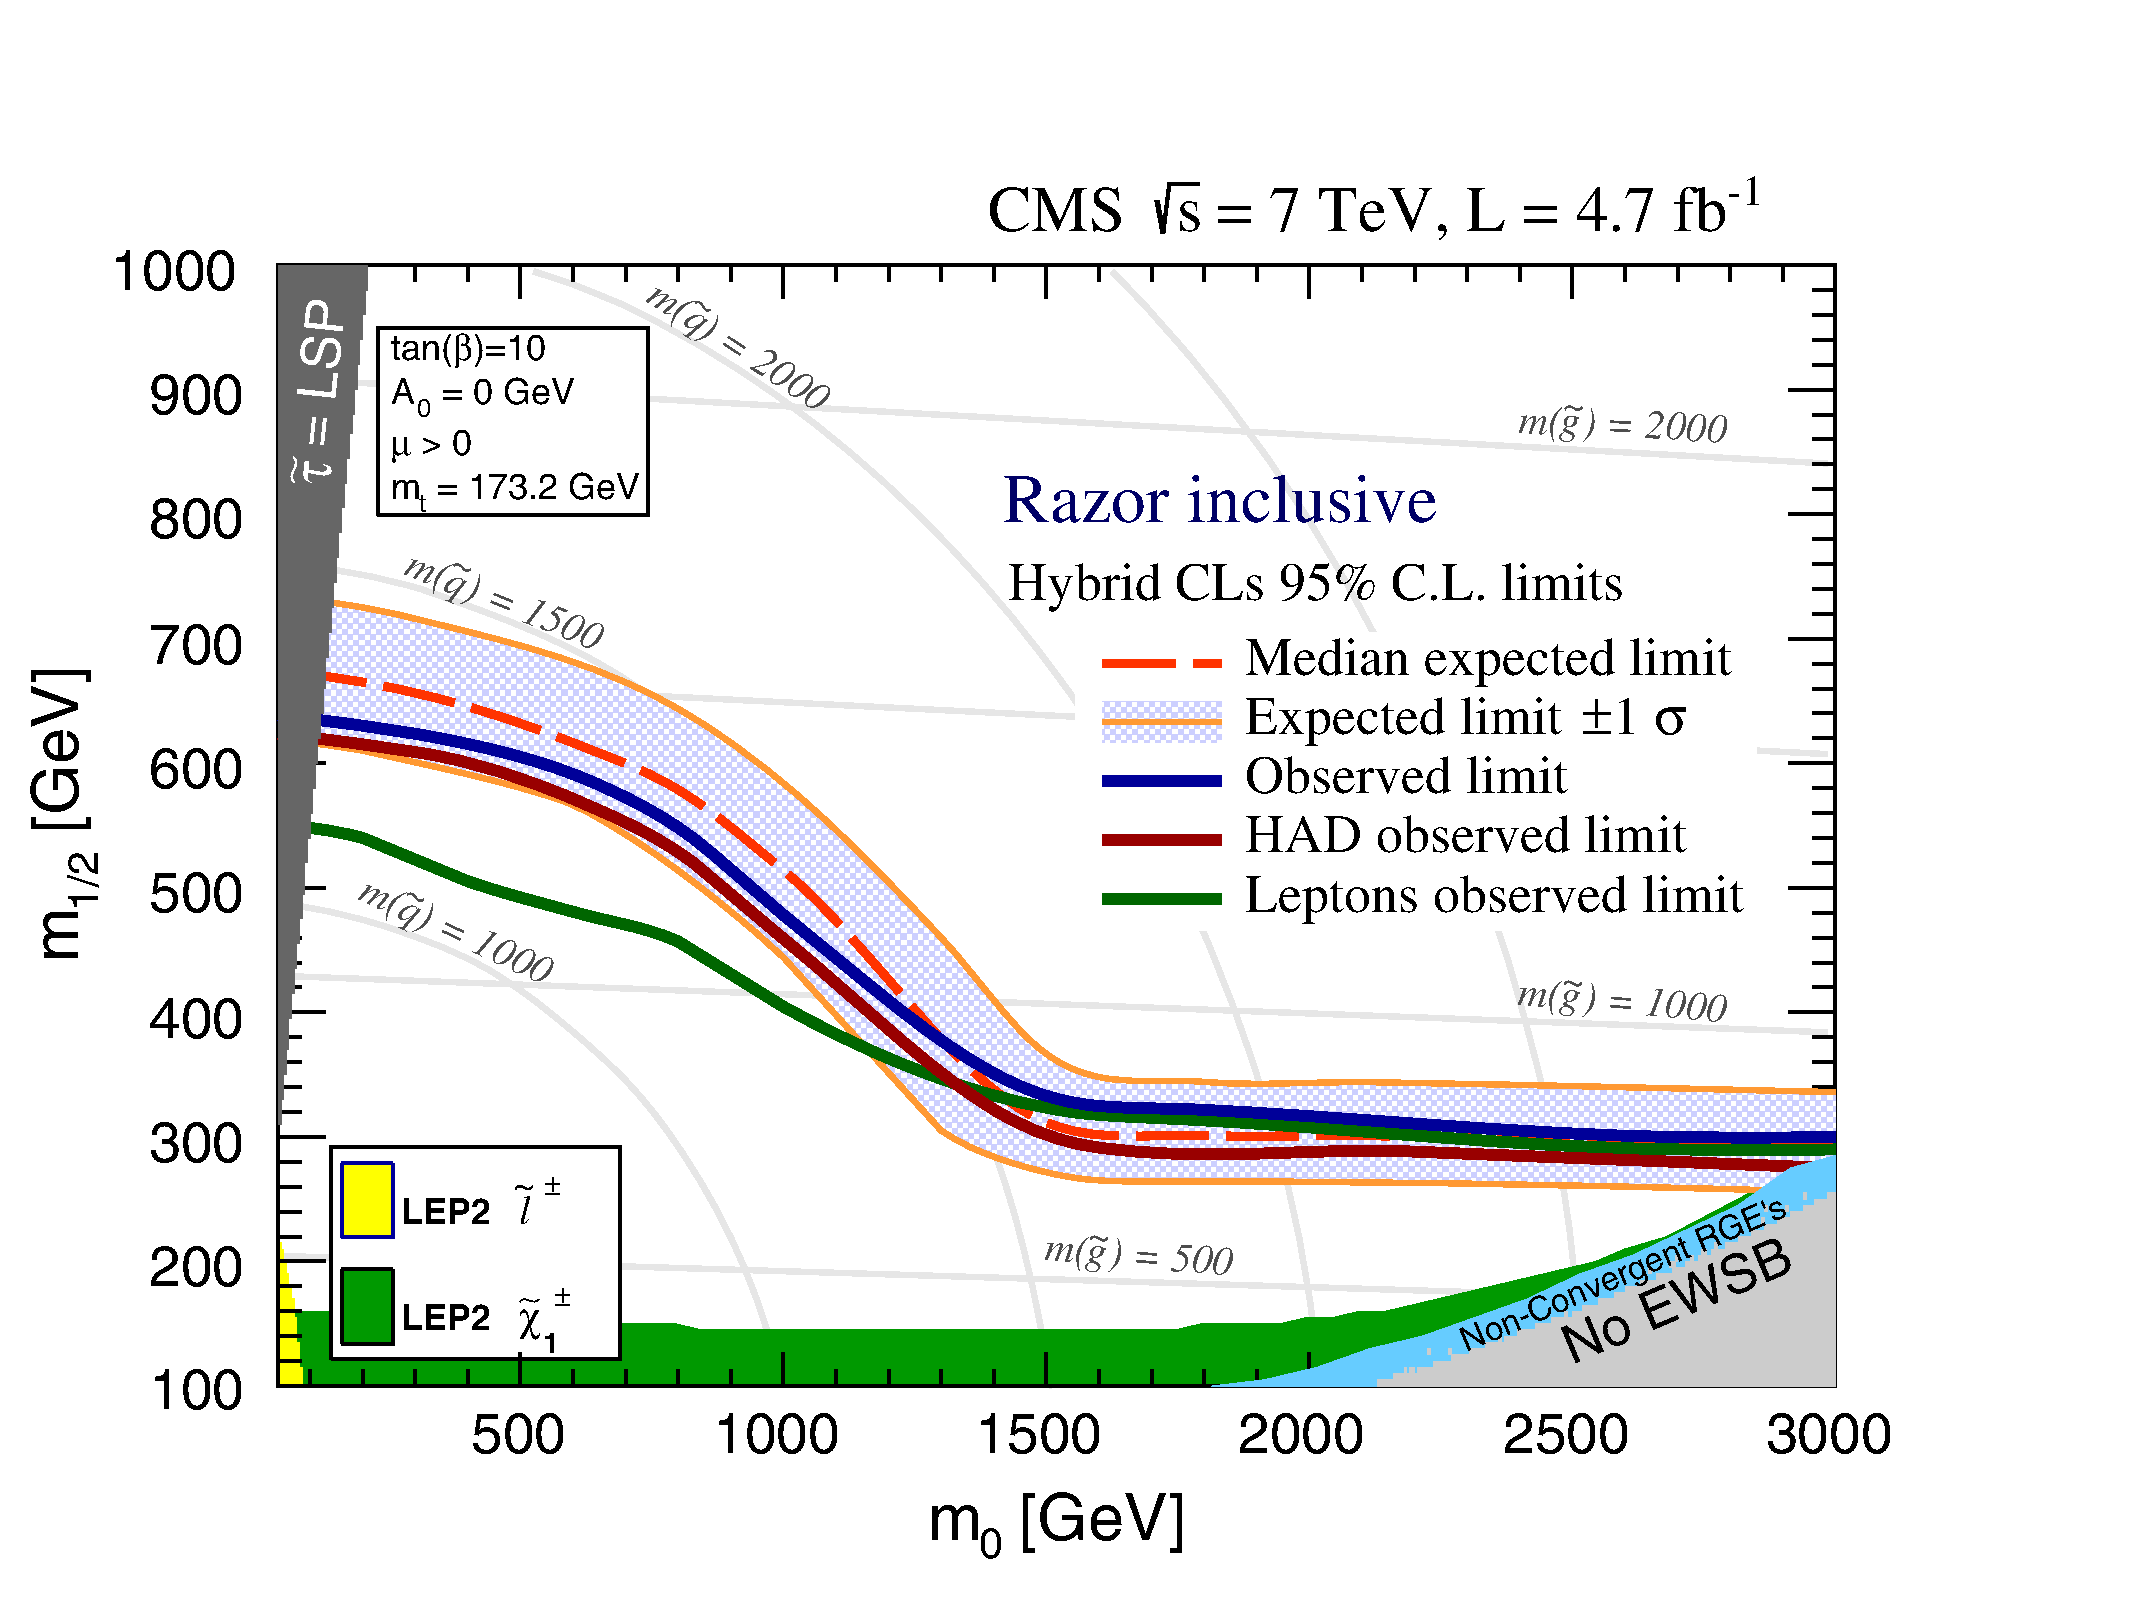
\includegraphics[width=0.7\textwidth]{RazorVariables/Limit7TeV.pdf}
\caption{Razor analysis 95\% CL. limit in the $m_{0}$-$m_{1/2}$
  plane of the CMSSM model using 7\TeV data. The model parameters have the following values: tan($\beta$) =
  10, $A_{0}$ = 0, and sign($\mu$) = +1.\label{fig:Limit7TeV}}
\end{figure} 

\begin{figure}
 \centering
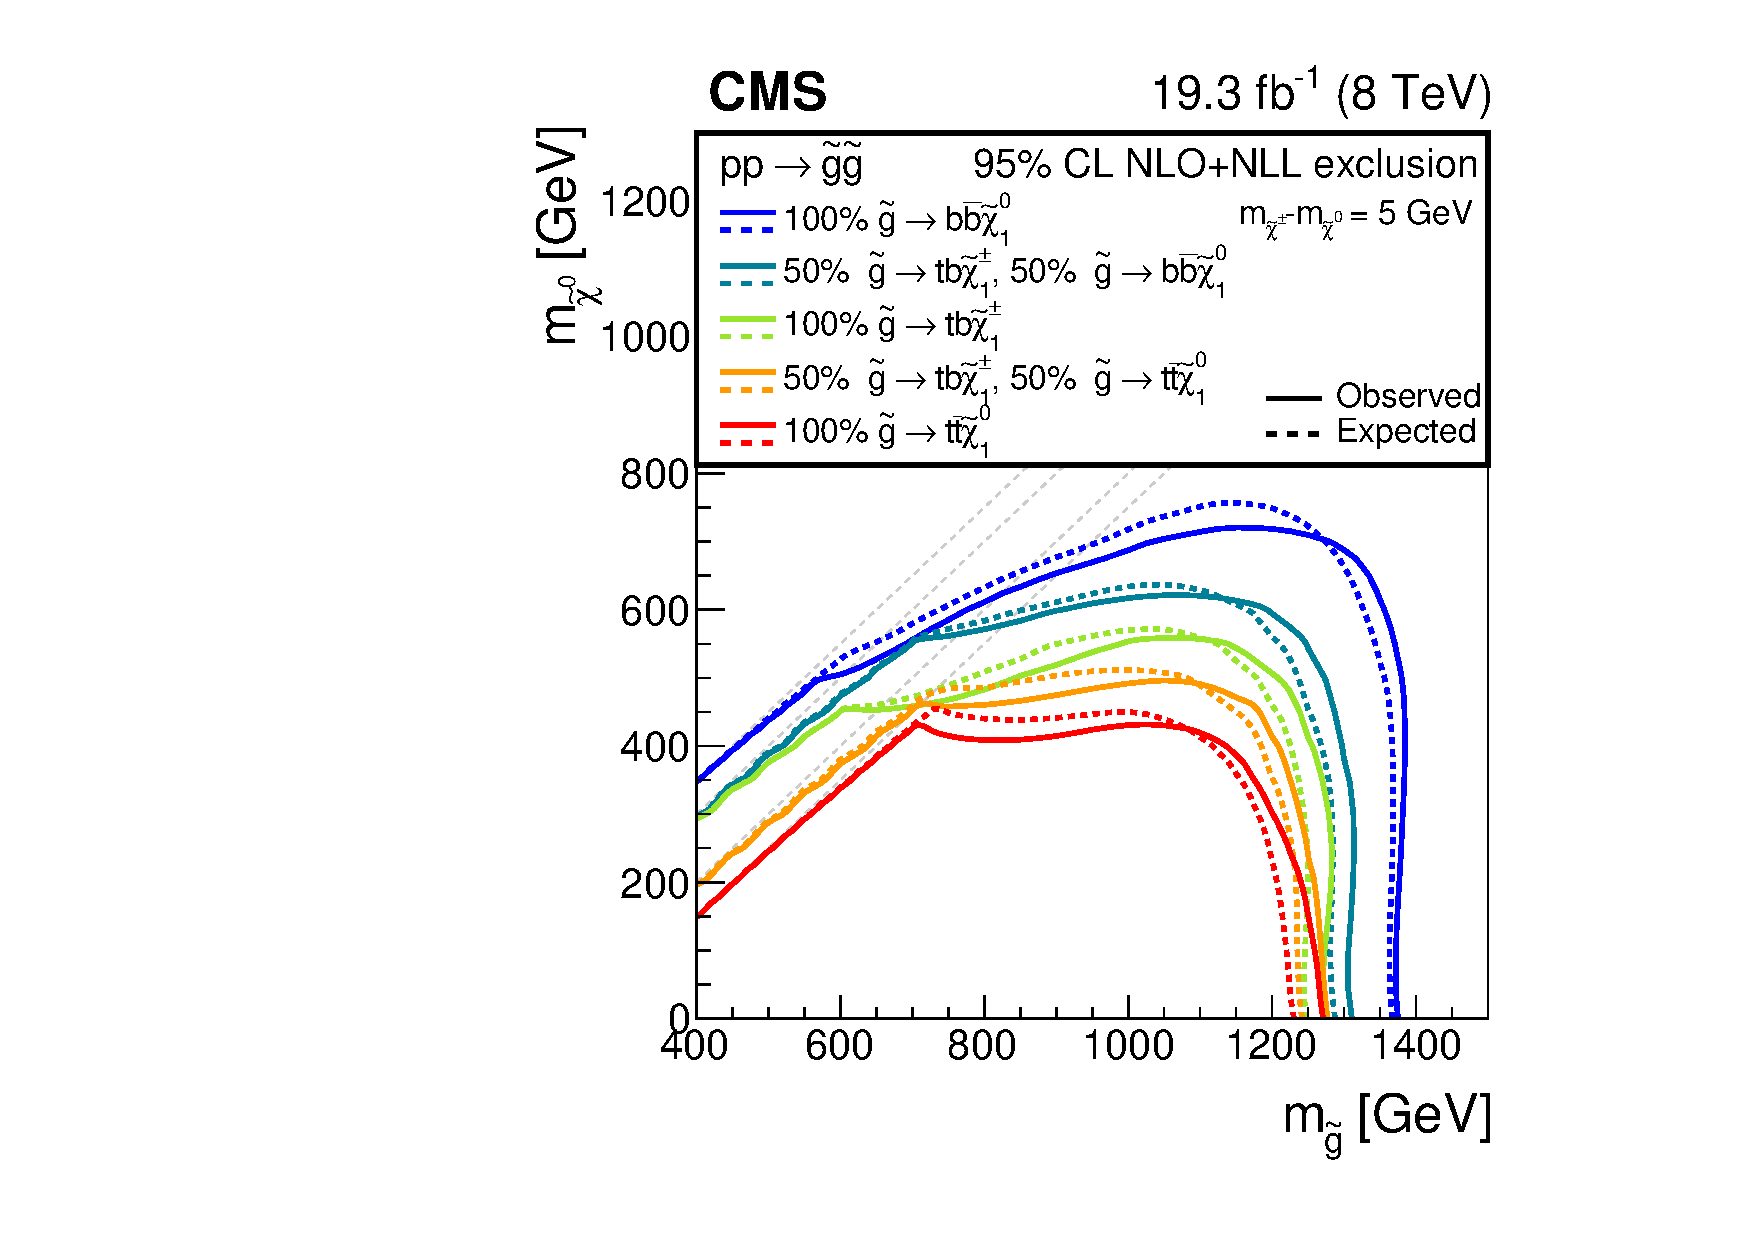
\includegraphics[width=0.49\textwidth]{RazorVariables/T1HybridNew0Lp1Lp2LBARE.pdf}
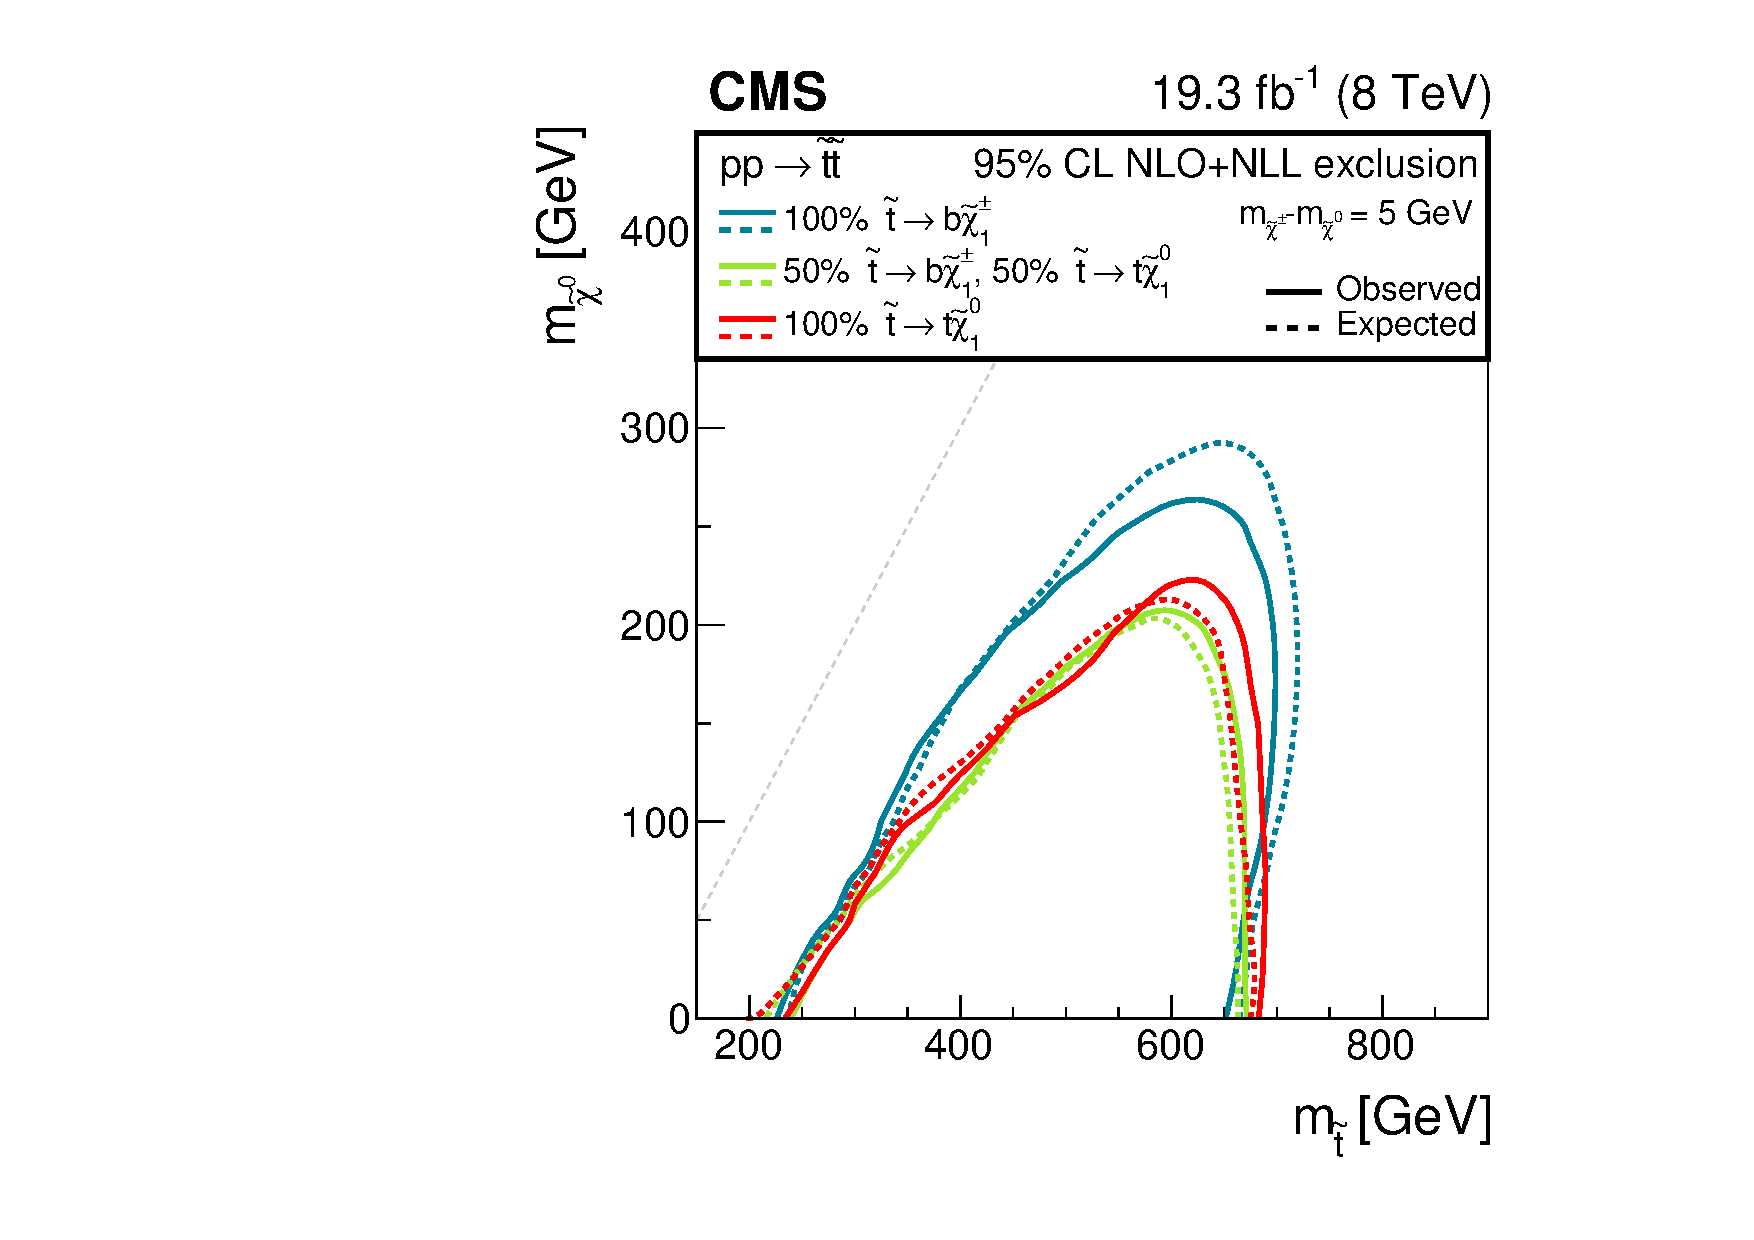
\includegraphics[width=0.49\textwidth]{RazorVariables/T2HybridNew0Lp1Lp2LBARE.pdf}
 \caption{Razor analysis 95\% CL. limits for (left) gluino and (right)
   stop pair-production using 8\TeV data. The limits are shown for
   different branching ratios of the particles involved.\label{fig:RazorLimit8TeV}}
\end{figure}

\begin{figure}
 \centering
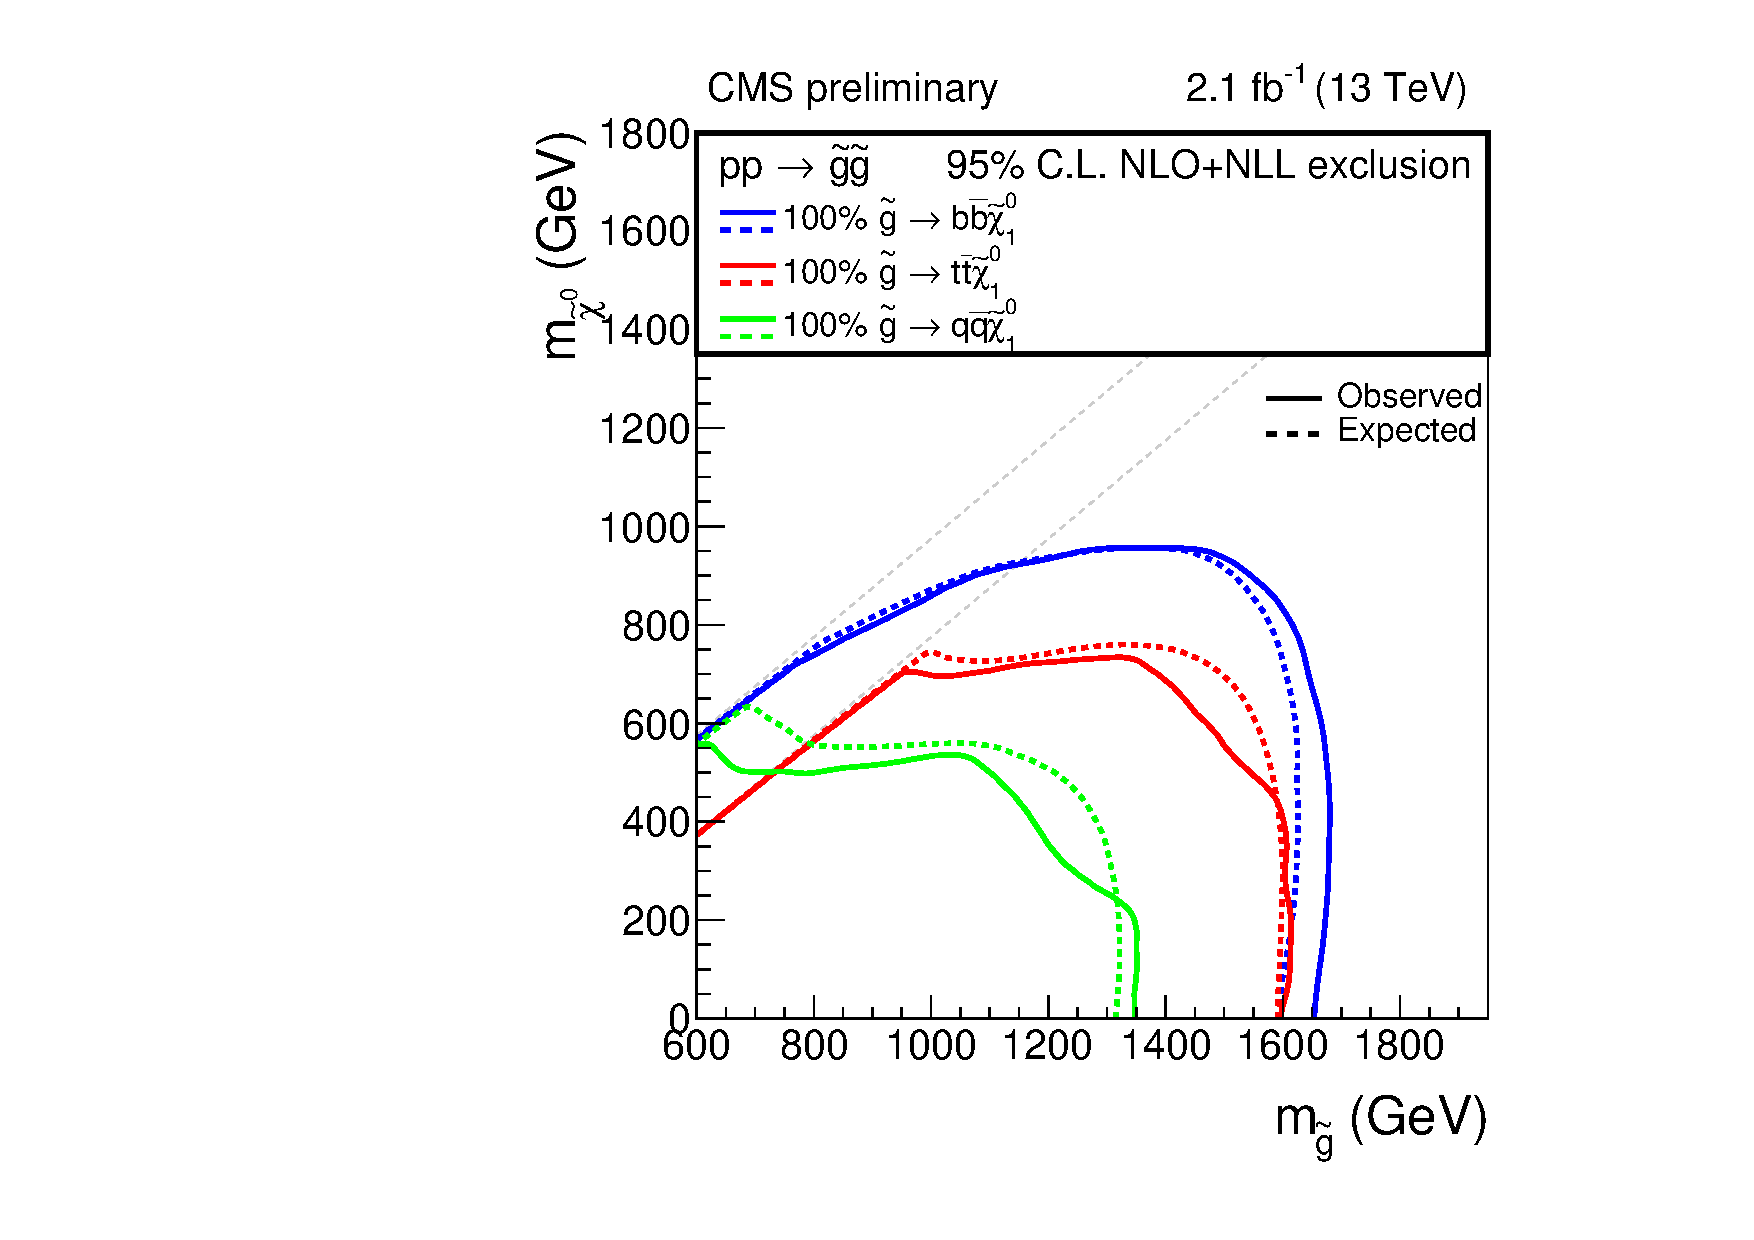
\includegraphics[width=0.7\textwidth]{RazorVariables/CMS-PAS-SUS-15-004_Figure_010.pdf}
\caption{Razor analysis 95\% CL. limits for gluino pair-production using 13\TeV data. The limits are shown for
   different branching ratios of the particles involved.\label{fig:RazorLimit13TeV}}
\end{figure} 

The razor approach has been taken beyond squark and gluino
pair-production to probe dark matter direct production and also
to look for possible anomalous production of Higgs bosons. Searches for dark matter direct
production have been a very hot topic at the LHC where the most common
final state includes a single high-$p_{\mathrm{T}}$  jet. It was
suggested that the razor variables could have comparable sensitivity
to dark matter direct production~\cite{Fox:2012ee} using a different kinematic
phase-space, since they require at least two jets, and therefore
increase the overall sensitivity to such a signal. Chapter~\ref{DMatLHC}
presents the CMS search that carries out this idea, confirming the
good sensitivity to direct dark matter production. Additionally, the razor
variables have been also used to search for anomalous Higgs production
by selecting events with jets and a diphoton pair whose invariant mass
is consistent with the Higgs mass. The first search of this kind was
carried out using the entire 8\TeV dataset~\cite{SUS-14-017} where an interesting excess
of events was observed at high values of $\mathrm{M_{R}}$ and the
results interpreted in the context of electroweak SUSY (see Section~\ref{hgg:8TeVsummary}). Chapter~\ref{HggRazor}
presents an updated result of this search with an entirely different
background estimation technique and using 15.3 fb$^{-1}$ of 13\TeV data.